\documentclass[12pt, letterpaper]{article}
\usepackage[toc,page]{appendix}
\usepackage[utf8]{inputenc}
\usepackage[pdftex]{graphicx}
\usepackage{xspace}
\usepackage[stable]{footmisc}
\usepackage{hyperref}
\usepackage{fullpage}
\usepackage{subcaption}
\usepackage{placeins}
\hypersetup{
    colorlinks=true,
    linkcolor=blue,
    filecolor=magenta,
    urlcolor=cyan,
}
\graphicspath{ {/home/tobiasjenegger/Documents/summary/} }
\title{GLAD analysis}
\author{Tobias Jenegger}
\date{}
\begin{document}
\begin{titlepage}
\maketitle
\end{titlepage}
\section{RUNS used for calibration = SWEEP RUNS without target}

\begin{center}
    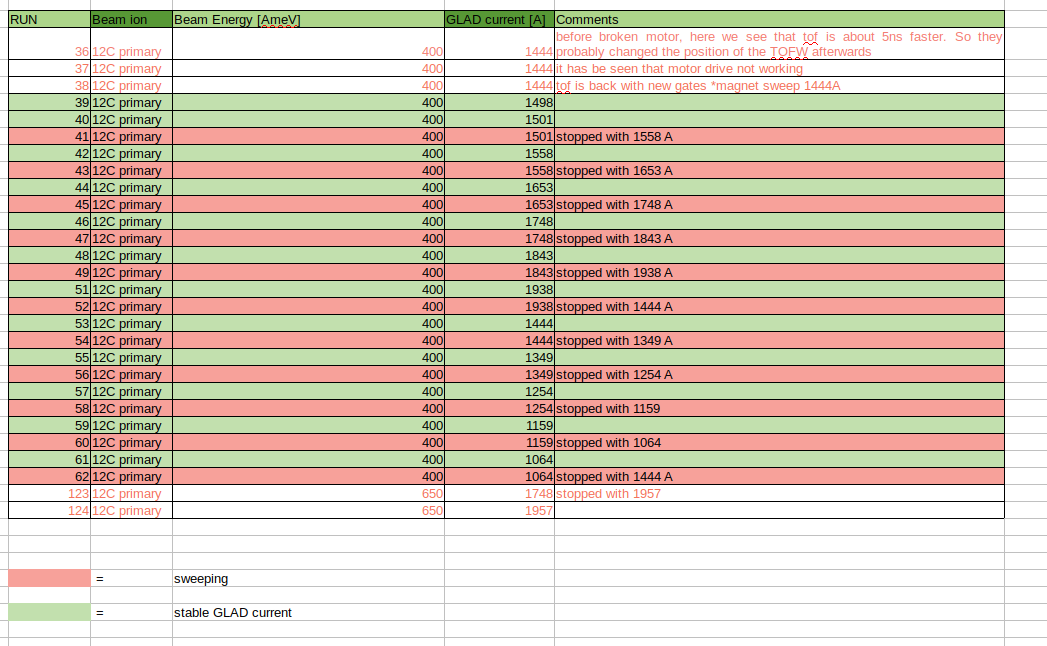
\includegraphics[width=1.0\textwidth]{runs_screenshot.png}
\end{center}
Run 62 could not be used to compare with RUN 53 (1444A), as the GLAD current was sweeping continuously from 1064 to 1444 Ampere.
\begin{figure}[!htbp]
\begin{subfigure}{.5\textwidth}
	\centering
	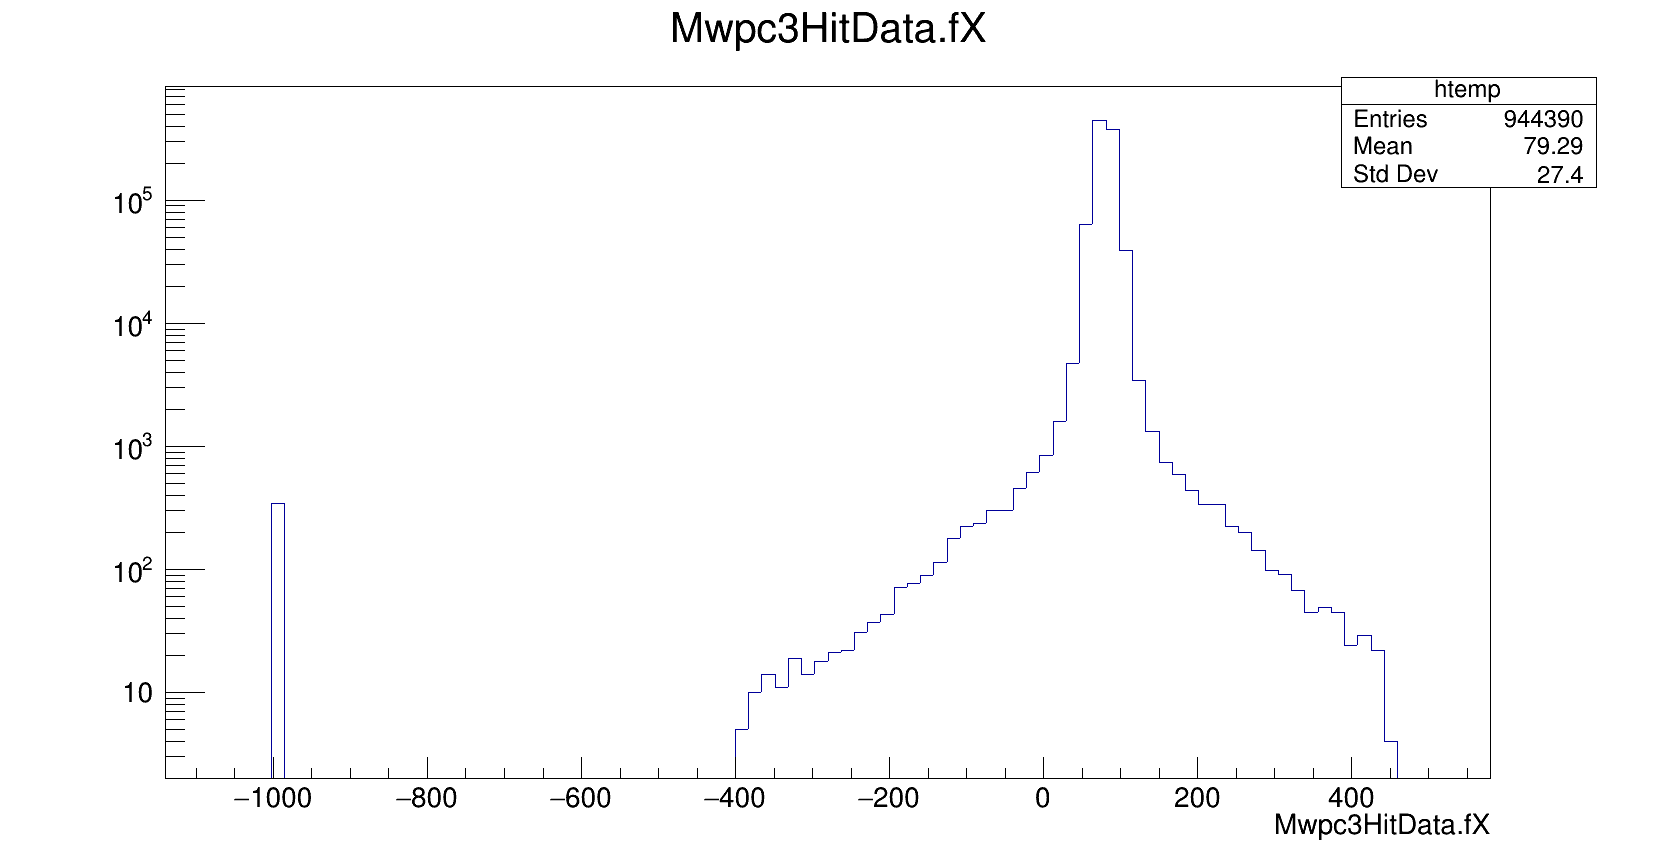
\includegraphics[width=.9\linewidth]{run53_mw3.png}
	\caption{"Event counts for MWPC3.fX in RUN 53 with GLAD current 1444A."}
	\label{fig:sub-second}
\end{subfigure}	
\begin{subfigure}{.5\textwidth}
	\centering
	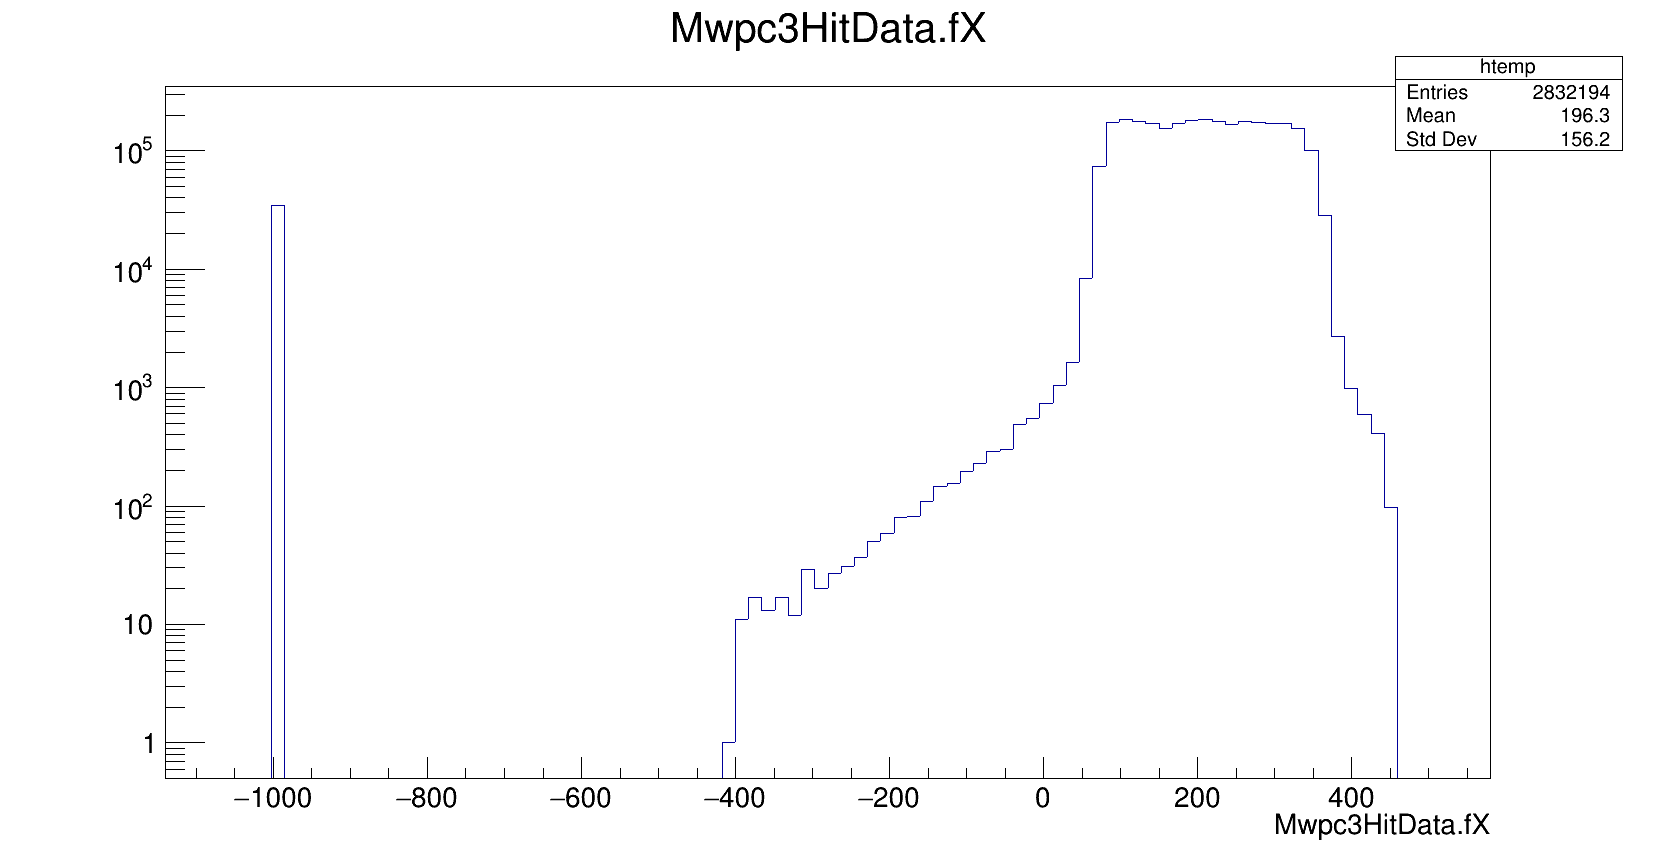
\includegraphics[width=.9\linewidth]{run62_mw3.png}
	\caption{"Event counts for MWPC3.fX in RUN 62 with sweeping GLAD current."}
	\label{fig:sub-second}
\end{subfigure}
\end{figure}
\begin{figure}[!htbp]
\begin{subfigure}{.9\textwidth}
	\centering
	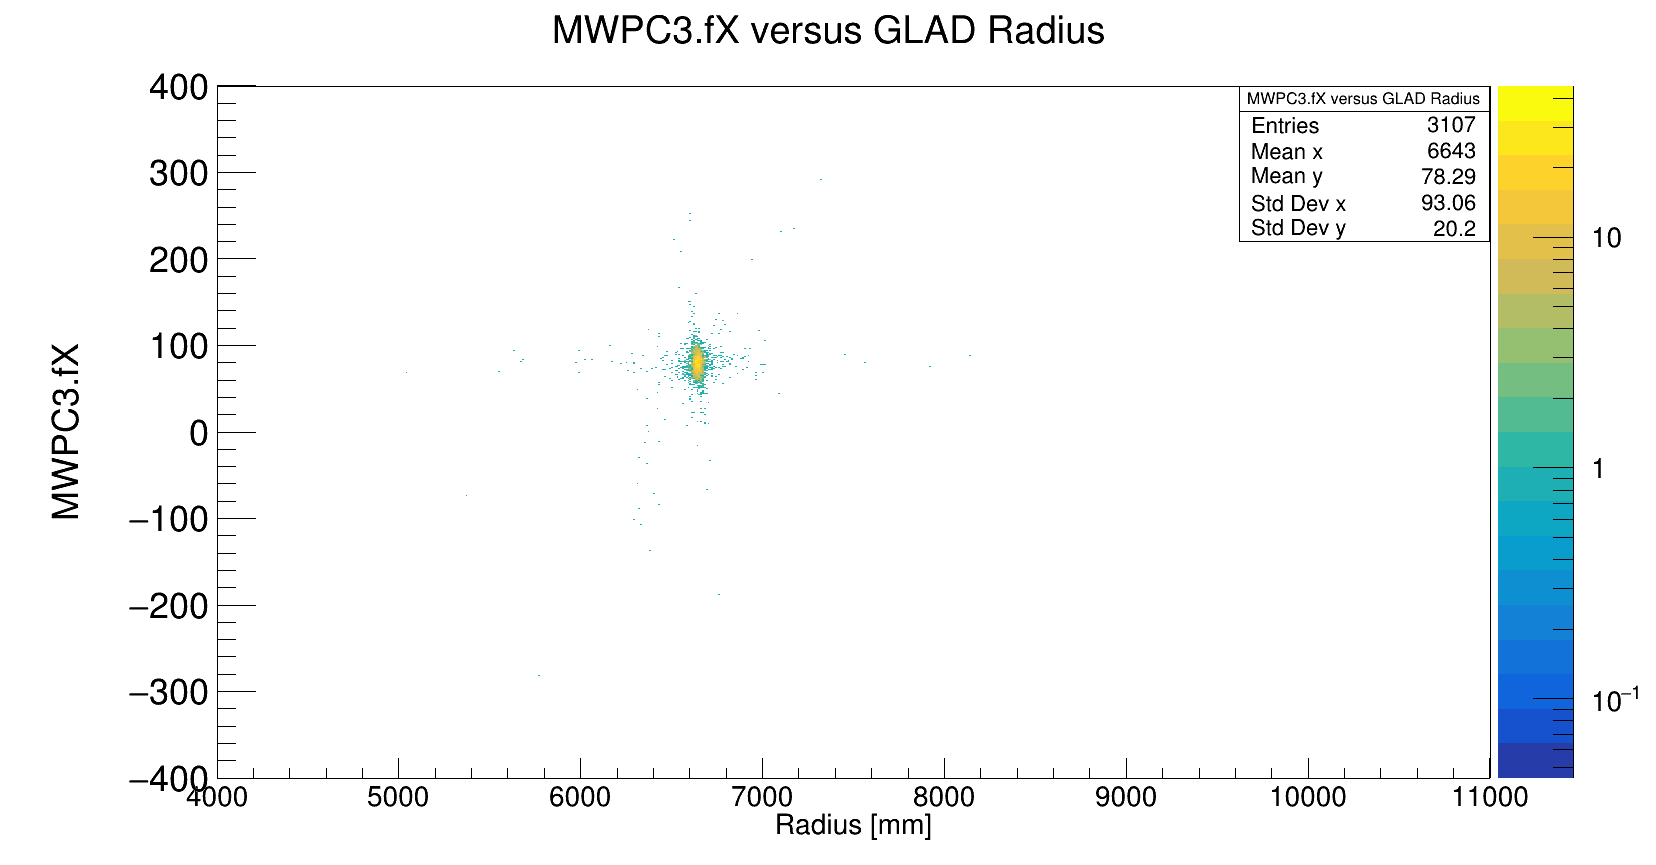
\includegraphics[width=.9\linewidth]{mw3_vs_rad_run53.png}
	\caption{"Radius vs MWPC3.fX for RUN 53 with GLAD current 1444A."}
	\label{fig:sub-second}
\end{subfigure}	
\begin{subfigure}{.9\textwidth}
	\centering
	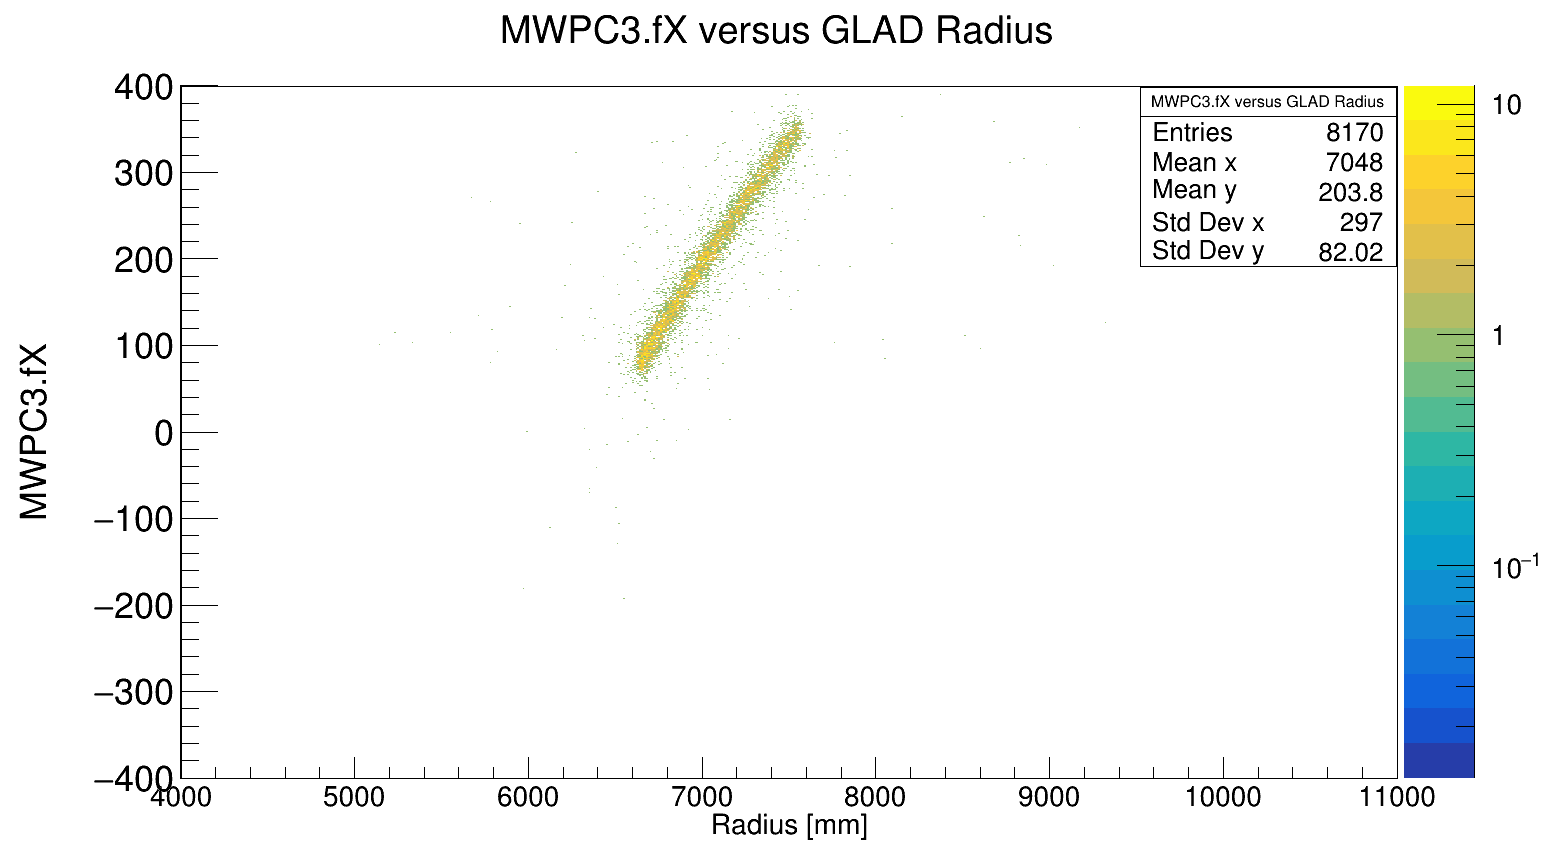
\includegraphics[width=.9\linewidth]{mw3_vs_rad_62.png}
	\caption{"Radius vs MWPC3.fX for RUN 62 with sweeping GLAD current."}
	\label{fig:sub-second}
\end{subfigure}
\end{figure}

Taking sweep RUNS 39-61 

\end{document}